%%%%%%%%%%%%%%%%%%%%%%%%%%%%%%%%%%%%%%%%%
%%%%%%%%%% Content starts here %%%%%%%%%%
%%%%%%%%%%%%%%%%%%%%%%%%%%%%%%%%%%%%%%%%%

\begin{frame}{Агенда}
	\begin{itemize}
	  \item Вовед
	  \item Мотивација
	  \item Хипотеза
	  \item Дизајн и имплементација
	  \item Идеи за идна работа
	  \item Заклучок
	\end{itemize}
\end{frame}

\begin{frame}{Што е Code?}
	\begin{itemize}
	  \item \emph{Code (E-Lab)} е веб-базиран систем за решавање задачи од
	  програмирање во почетни курсеви за програмирање
	  \item Целокупнота работа е во веб прелистувач
	  \item Заштитено извршување (Sandbox)
	  \item Подржува различни програмски јазици (C, C++, Java, Python)
	  \item Лесно надградлив и скалабилен
	\end{itemize}
\end{frame}

\begin{frame}{Мотивација}
    \begin{itemize}
      \item Програмирањето е една од основните практични вештини која што се
      изучува во програмите на информатичките факултети и секундарна вештина на
      многу други технички факултети
      \item Големата побарувачка на пазарот на трудот за програмери е една од
      причините за интересот и популарноста меѓу идните студенти
      \item Резултат се големи групи студенти во воведните курсеви
      \item Но програмирањето не е лесно!
      \item Потребно е да се решат голем број основни алгоритамски проблеми
      (повеќе од една третина од времето)
    \end{itemize}
\end{frame}


% Define block styles
\tikzstyle{block} = [rectangle, draw, fill=blue!20,
text width=5em, text centered, rounded corners, minimum height=4em]
\tikzstyle{line} = [draw, -latex']

\begin{frame}[fragile]{Основата на Code}
    \begin{itemize}
      \item Алгоритамски видови на задачи
    \end{itemize}
\begin{center}
\begin{tikzpicture}[node distance = 3cm, auto]
    % Place nodes
    \pause
    \node [block] (input) {Влез};
    \pause     
    \path [line] (input) -> node {} (algorithm);
    \node [block, right of=input] (algorithm) {Алгоритам}
    \pause
    \path [line] (algorithm) -> node {} (output);
    \node [block, right of=algorithm] (output) {Излез};
    % Draw edges
\end{tikzpicture}
\end{center}
\pause
\begin{itemize}[<+->]
  \item Се користи во системи за натпревари во програмирање
  \item Ја потенцираат важноста во програмирањето да се има решение
  кое работи точно
\end{itemize}
\end{frame}


\begin{frame}{Хипотеза}
    \begin{itemize}
      \item Со помош на напредни веб-базирани алатки може да се подобри, олесни
      и потпомогне пишувањето програми
      \item Примената на современи методи за едукација ќе ја зголеми
      мотивираноста на студентите изучување програмирање и совладување
      на основните концепти
      \item Веб-базираната имплементација на овие алатки треба да овозможи
      поголема достапност на алатките
      \item Масовна употреба на овие алатки, може да помогне во идентификација
      на проблемите и потешкотиите во изучување програмирање кај почетници
    \end{itemize}
\end{frame}

\begin{frame}{Предложена методологија}
    \begin{itemize}
      \item Прашалници и анкети
      \item Обработка на статистиката за користење
      \item Анализа и споредба на резултатите 
      \item Издвојување на контролна група
    \end{itemize}
    Седум принципи на добра практика (Chickering
and Gamson (1987))
    \begin{enumerate}
      \item Контакт помеѓу студентот и факултетот
      \item Соработка меѓу студентите
      \item Активно учење
      \item Навремени одговори
      \item Нагласување на временските ограничувања
      \item Соопштување на високите очекувања
      \item Почитување на различностите во талентот и начините на учење
    \end{enumerate}
\end{frame}

\begin{frame}{Дизајн и имплементација на системот}
    \begin{figure}
    \centering
        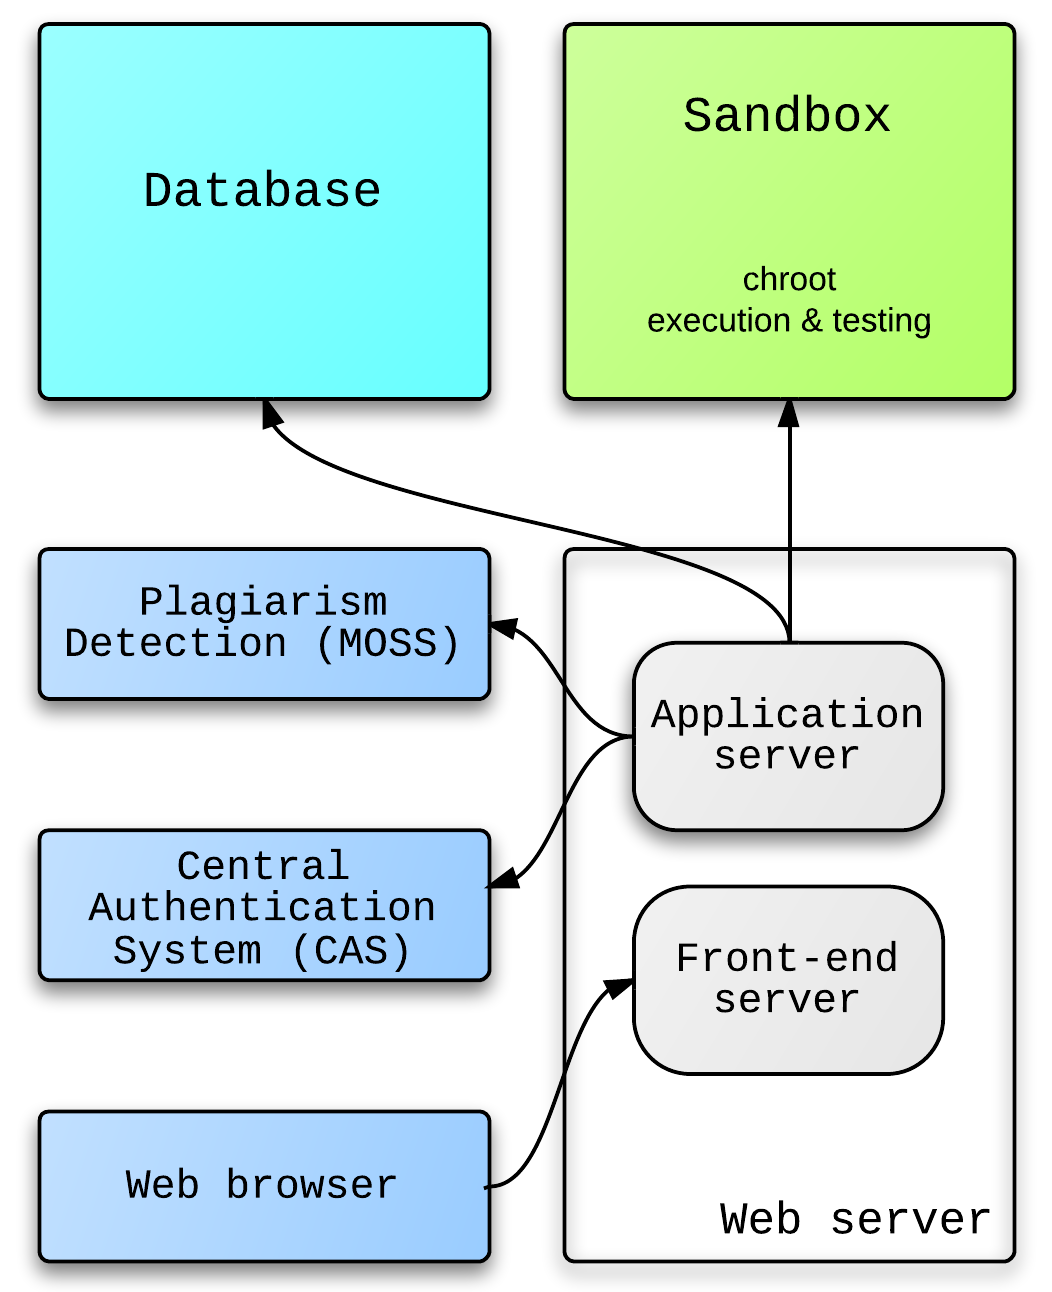
\includegraphics[width=.35\textwidth]{images/architecture-new}
        \caption{Архитектура на системот.}
        \label{fig:architecture}
    \end{figure}
\end{frame}

\begin{frame}{Интегриран поглед на задача}
    \begin{figure}
    \centering
        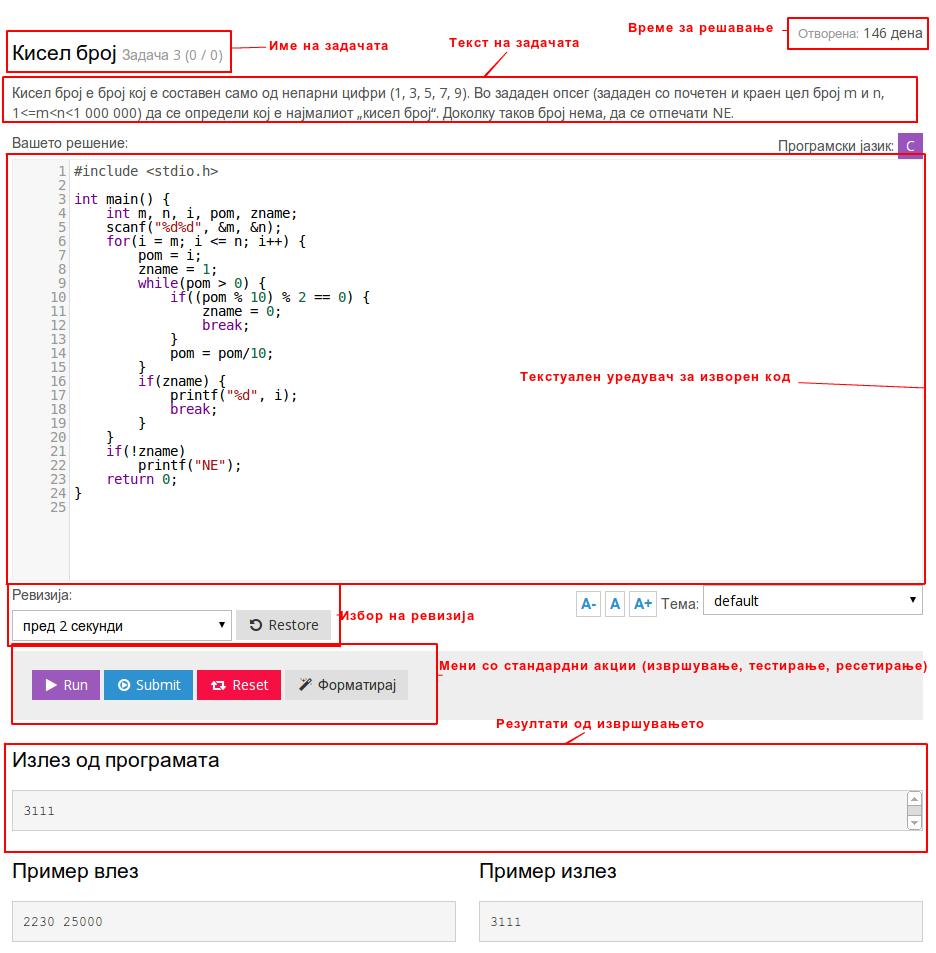
\includegraphics[width=.6\textwidth]{images/integrated_code_view}
        \label{fig:architecture}
    \end{figure}
  \end{frame}


\begin{frame}{Податоци за користење}{Корисници}
\begin{itemize}
  \item 1498 корисници
    \begin{itemize}
    \item 1350 студенти
    \item 36 инструктори
    \item 10 наставници и асистенти
    \item 2 администратори
    \end{itemize}
\end{itemize}
\end{frame}

\begin{frame}{Податоци за користење}{Курсеви}
Моментално се активни четири курсеви од зимскиот семсетар
\begin{enumerate}
  \item Концепти за развој на софтвер (I година, 692 студенти)
  \item Алгоритми и структури на податоци (II година, 545 студенти)
  \item Напредно програмирање (II година, 75 студенти)
  \item Структурирано програмирање (I година, 80 студенти)
\end{enumerate}
и четири курсеви од летниот семестар:
\begin{enumerate}
  \item Напреден развој на софтвер (I година, 630 студенти)
  \item Објектно-ориентирано програмирање (I година, 74 студенти)
  \item Напредни алгоритми (II година, 24 студенти)
  \item Објектно и визуелно програмирање (I година, 105 студенти)
\end{enumerate}
\end{frame}

\begin{frame}{Податоци за користење}{Задачи и решенија}
\begin{itemize}
  \item Досега се креирани 539 задачи во 111 групи (вежби, испити, домашни)
  \item Забележани се 204066 обиди за решавање, од кои 77087 се точни (38\%)
  \item Просечниот број на обиди по задача е 414
  \item Досега на системот успешно и без проблеми се одржани 10 колоквиуми и 3
  испити
\end{itemize}
\end{frame}

\begin{frame}{Плагијаризам}
\begin{itemize}
  \item Направена е анализа за плагијaризмот во рамките на два предмети \textbf{Концепти за
развој на софтвер (C)} и \textbf{Напредно програмирање (Java)}
\item Системот за детекција на плагијати MOSS
\item Кај задачите од лабораториски вежби („контролирана средина“) забележани се
бројни плагијати (на некои задачи и преку 30\%)
\item Кај испитите и колоквиумите не се забележани случаи на плагијати
\item Постојат и позитивни примери на индивидуални домашни работи
\end{itemize}
\end{frame}


\begin{frame}{Идеи за понатамошни истражувања}
\begin{itemize}
  \item Следење и визуелизација на извршувањето
  \item Појаснување и дополнително објаснување на грешките
  \item Интеграција со систем за учење
  \item Далечинска контрола и колаборација во реално време
  \item Можности за персонализација
  \item Архитектура за имплементација во облак и зголемена скалабилност
\end{itemize}
\end{frame}

\begin{frame}{Заклучок}
    \begin{itemize}
      \item Code од идеја, до реализација на веб-базирана околина за
      програмирање
      \item Преку имплементација, тестирање и примена на современи
      методолгии се овозможува истражување во компјутерската едукација
      \begin{itemize}
        \item Со посебен аспект на програмирање и пишување алгоритми
      \end{itemize}
      \item Приклучок кон светските трендови на приближување
      на образованието кон поголема маса на луѓе, со користење на најновите
      технологии
    \end{itemize}
\end{frame}

\begin{frame}{Прашања}{}
    \begin{center}
    \Large{
    \href{http://code.finki.ukim.mk/}{\textbf{http://code.finki.ukim.mk}}}
    \vfill
    \huge{Ви благодарам на вниманието}
    \vfill    
    \Huge{Прашања?}
    \end{center}
\end{frame}







